% !TEX root = ../../../main.tex

\begin{note}
    Выведем интуицию, связывающую Хёффдинга из интегральной теоремы Муавра--Лапласа. Пусть \(\xi \sim Bin(n, p)\).
    \[P(\xi_n \ge a) = P\left( \sum_{i = 1}^n \eta_i \ge a\right) = P\left( \sum_{i = 1}^n \frac{\eta_i + 1}{1} \ge \frac{a + n}{2} \right) = (*)\]
    Положим \(\phi_i = \left\{\begin{array}{l}
        1, \text{ с вероятностью \(p\)} \\
        0, \text{ с вероятностью \(q\)} \\
    \end{array}\right.\).
    Тогда:
    \[(*) = P\left( \sum_{i = 1}^n \phi_i \ge \frac{a + n}{2} \right) = P\left( \frac{\sum_{i = 1}^n \phi_n - \frac{n}{2}}{\sqrt{n/4}} \ge \frac{a/2}{\sqrt{n/4}}\right)\sim \frac{1}{2\pi}\int_{\frac{a}{\sqrt{n}}}^{+\infty}e^{-\frac{x^2}{2}} \approx e^{-\frac{a^2}{2n}}\]
\end{note}

\begin{theorem}
    Пусть \(p = \frac{c}{n}, c > 0\).
    \begin{enumerate}
        \item Если \(c < 1\), то \(\exists \beta(c)\), такая, что а.п.н. каждая компонента \(G(n, p)\) имеет \(\le \beta \ln n\) вершин.
        \item Если \(c > 1\), то \(\exists \beta(c), \gamma(c) \in (0, 1)\), такие, что а.п.н. в \(G(n, p)\) есть ровно одна компонента в которой \(\ge \gamma n\) вершин, а все остальные компоненты связности имеют \(\le \beta \ln n\) вершин.
    \end{enumerate}
\end{theorem}

\begin{figure}[h!]
    \begin{center}
        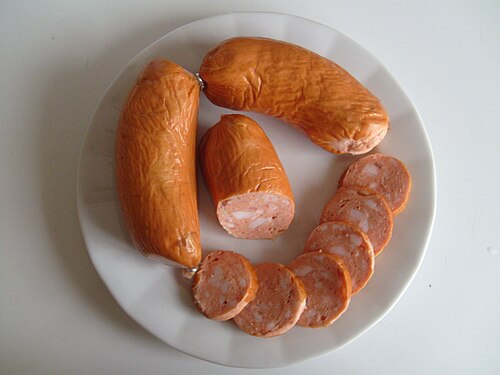
\includegraphics[scale=0.3]{images/shpikachka.jpg}
    \end{center}
    \caption{Шпикачка}
\end{figure}
\begin{proof}
    Запустим процесс: будем по очереди оживлять вершины. Пусть в момент времени \(t\), \(Y_t\) --- число живых вершин, \(Z_t\) --- число потомков живых вершин, \(N_t\) --- число нейтральных вершин. Тогда:
    \[Y_0 = 1, N_0 = n - 1, Z_1 \sim Bin(n - 1, p)\]
    \[Y_t = Y_{t - 1} + Z_t - 1, N_0 = n - 1, Z_1 \sim Bin(n - 1, p), Z_t \sim Bin(N_{t - 1}, p)\]
    \[Y_t + N_t + t = n\]

    \begin{lemma}
        \(Y_t = 1 - t + Bin(n - 1, 1 - (1 - p)^t)\)
    \end{lemma}
    \begin{proof}
        \[Y_t + N_t + t = n\]
        \[N_t = n - 1 + 1 - t - Y_t = 1 - t + (n - 1 - Y_t)\]
        Но тогда
        \[Y_t = 1 - t + Bin(n - 1, 1 - (1 - p)^t) \Lra N_t = Bin(n - 1, (1 - p)^t)\]
        Докажем последнее равенство по индукции по \(t\).
        \begin{enumerate}
            \item[] \textbf{База:} \(t = 0\), \(N_0 \sim Bin(n - 1, 1)\).
            \item[] \textbf{Переход:} 
            \[Y_{t - 1} + N_{t - 1} + t - 1 = n \Ra Y_{t - 1} = n - (t - 1) - N_{t - 1}\]
            \[N_t = n - 1 - t + 1 - Y_t = (n - 1) - (t - 1) - Y_{t - 1} - Z_t + 1 = (n - 1) - (t - 1) - n + N_{t - 1} + (t - 1) - Z_t + 1 = N_{t - 1} - Z_t = N_{t - 1} - Bin(N_{t - 1}, p) = Bin(N_{t - 1}, 1 - p)\]
            По предположению индукции, \(N_{t - 1} = Bin(n - 1, (1 - p)^{t - 1})\), тогда:
            \[N_t = Bin(N_{t - 1}, 1 - p) = Bin(n, (1 - p)^t)\]
        \end{enumerate}
    \end{proof}

    \[P(\text{существует компонента связности с \(\ge \beta \ln n\) вершинами}) \le\]
    \[P(\text{существует вершина, такая, что \(Y_t > 0\) при \(t = \beta \ln n\)}) \le nP(Y_t > 0) = \]
    \[ = nP(Bin(n - 1, 1 - (1 - p)^t) \ge t) \le nP(Bin(n - 1, pt) \ge t) = (*)\]
    Помним, что \(p = \frac{c}{n}, c < 1\).


    \begin{theorem}[б/д]
        Пусть \(p = \frac{c}{n}, c < 1\). Тогда \(P(Binom(n, pt) \ge t) \le e^{-\gamma t}, \gamma = \gamma(c) > 0\).
    \end{theorem}
    \begin{proof}[Пояснение с использованием теоремы Муавра-Лапласа]
        \[P\left( \frac{Bin(n, pt) - npt}{\sqrt{npt(1 - pt)}} \ge \frac{\overbrace{t - npt}^{t(1 - c)}}{\sqrt{npt(1 - pt)}} \right) \sim \frac{1}{\sqrt{2\pi}}\int_{\frac{t(1 - c)}{\sqrt{npt(1 - pt)}}}^{+\infty}e^{-\frac{x^2}{2}}dx \approx e^{-\frac{(t(1 - c))^2}{2npt(1 - pt)}} \le e^{-\gamma t}\]
    \end{proof}

    Но тогда 

    \[(*) \le nP(Bin(n, pt) \ge t) \le ne^{-\gamma t} \le ne^{\gamma \beta\ln n} = \frac{n}{n^{\gamma\beta}}\]
    Причем можно выбрать \(\beta\) так, что \(\frac{n}{n^{\gamma\beta}} \ra 0 \Ra\) утвеждение доказано
\end{proof}

\subsection{Хроматическое число случайного графа}
\begin{theorem}
    \begin{enumerate}
        \item Если \(p = o\left( \frac{1}{n^2} \right)\), то а.п.н. \(\chi(G) = 1\)
        \item Если \(pn^2 \ra \infty\), но \(p = o\left( \frac{1}{n} \right)\), то а.п.н. \(\chi(G) = 2\)
        \item Если \(p = \frac{c}{n}, c < 1\), то а.п.н. \(\chi(G) = 3\).
    \end{enumerate}
\end{theorem}